%to have line numbers
%\RequirePackage{lineno}
\documentclass[10pt, letterpaper]{article}      
\usepackage[margin=.1cm,font=small,labelfont=bf]{caption}[2007/03/09]
%\usepackage{endnotes}
%\let\footnote=\endnote
\usepackage{setspace}
\usepackage{longtable}                        
\usepackage{anysize}                          
\usepackage{natbib}                           
%\bibpunct{(}{)}{,}{a}{,}{,}                   
\bibpunct{(}{)}{,}{a}{}{,}                   
\usepackage{amsmath}
\usepackage[% draft,
pdftex]{graphicx} %draft is a way to exclude figures                
\usepackage{epstopdf}
\usepackage{hyperref}                             % For creating hyperlinks in cross references
\hypersetup{pdfborder={0 0 0.4}} %have nice light boxes on refs
 
% \usepackage[margins]{trackchanges}

% \note[editor]{The note}
% \annote[editor]{Text to annotate}{The note}
%    \add[editor]{Text to add}
% \remove[editor]{Text to remove}
% \change[editor]{Text to remove}{Text to add}

%TODO make it more standard before submission: \marginsize{2cm}{2cm}{1cm}{1cm}
\marginsize{1cm}{1cm}{.5cm}{.5cm}%{left}{right}{top}{bottom}   
					          % Helps LaTeX put figures where YOU want
 \renewcommand{\topfraction}{1}	                  % 90% of page top can be a float
 \renewcommand{\bottomfraction}{1}	          % 90% of page bottom can be a float
 \renewcommand{\textfraction}{0.0}	          % only 10% of page must to be text

 \usepackage{float}                               %latex will not complain to include float after float

\usepackage[table]{xcolor}                        %for table shading
\definecolor{gray90}{gray}{0.90}
\definecolor{orange}{RGB}{255,128,0}

\renewcommand\arraystretch{.9}                    %for spacing of arrays like tabular

%-------------------- my commands -----------------------------------------
\newenvironment{ig}[1]{
\begin{center}
 %\includegraphics[height=5.0in]{#1} 
 \includegraphics[height=3.3in]{#1} 
\end{center}}

 \newcommand{\cc}[1]{
\hspace{-.13in}$\bullet$\marginpar{\begin{spacing}{.6}\begin{footnotesize}\color{blue}{#1}\end{footnotesize}\end{spacing}}
\hspace{-.13in} }

%-------------------- END my commands -----------------------------------------



%-------------------- extra options -----------------------------------------

%%%%%%%%%%%%%
% footnotes %
%%%%%%%%%%%%%

%\long\def\symbolfootnote[#1]#2{\begingroup% %these can be used to make footnote  nonnumeric asterick, dagger etc
%\def\thefootnote{\fnsymbol{footnote}}\footnote[#1]{#2}\endgroup}	%see: http://help-csli.stanford.edu/tex/latex-footnotes.shtml

%%%%%%%%%%%
% spacing %
%%%%%%%%%%%

% \abovecaptionskip: space above caption
% \belowcaptionskip: space below caption
%\oddsidemargin 0cm
%\evensidemargin 0cm

%%%%%%%%%
% style %
%%%%%%%%%

%\pagestyle{myheadings}         % Option to put page headers
                               % Needed \documentclass[a4paper,twoside]{article}
%\markboth{{\small\it Politics and Life Satisfaction }}
%{{\small\it Adam Okulicz-Kozaryn} }

%\headsep 1.5cm
% \pagestyle{empty}			% no page numbers
% \parindent  15.mm			% indent paragraph by this much
% \parskip     2.mm			% space between paragraphs
% \mathindent 20.mm			% indent math equations by this much

%%%%%%%%%%%%%%%%%%
% extra packages %
%%%%%%%%%%%%%%%%%%

\usepackage{datetime}


\usepackage[latin1]{inputenc}
\usepackage{tikz}
\usetikzlibrary{shapes,arrows,backgrounds}


%\usepackage{color}					% For creating coloured text and background
%\usepackage{float}
\usepackage{subfig}                                     % for combined figures

\renewcommand{\ss}[1]{{\colorbox{blue}{\bf \color{white}{#1}}}}
\newcommand{\ee}[1]{\endnote{\vspace{-.10in}\begin{spacing}{1.0}{\normalsize #1}\end{spacing}\vspace{.20in}}}
\newcommand{\emd}[1]{\ExecuteMetaData[/tmp/tex]{#1}} % grab numbers  from stata

%TODO before submitting comment this out to get 'regular fornt'
\usepackage{sectsty}
\allsectionsfont{\normalfont\sffamily}
\usepackage{sectsty}
\allsectionsfont{\normalfont\sffamily}
\renewcommand\familydefault{\sfdefault}

%\usepackage[margins]{trackchanges}
\usepackage{rotating}
\usepackage{catchfilebetweentags}

\usepackage{abstract}
\renewcommand{\abstractname}{}    % clear the title
\renewcommand{\absnamepos}{empty} % originally center
%-------------------- END extra options -----------------------------------------
\date{{}\today \hspace{.2in}\xxivtime}
\title{  % remember to have Vistula University!!
  The Impact of Covid19\\ on\\ the Urban-Rural Happiness %Gradient
}
\author{
% Adam Okulicz-Kozaryn\thanks{EMAIL: adam.okulicz.kozaryn@gmail.com
%   % \hfill I thank XXX.  All mistakes are mine.
% } \\
% {\small Rutgers - Camden  % and Vistula University
% }\\
% Rubia R. Valente\\
% {\small CUNY/Baruch}
}

\begin{document}

%%\setpagewiselinenumbers
%\modulolinenumbers[1]
%\linenumbers

\bibliographystyle{/home/aok/papers/root/tex/ecta}
\maketitle
\vspace{-.4in}
\begin{center}

\end{center}

\textbf{abstract:}
\begin{abstract}
  \noindent People tend to be less happy in cities than in rural areas, the so called ``urban-rural happiness gradient.'' The recent covid19
  pandemic allows us to explore one of the  disadvantages of
  large and dense cities: the faster spread of infectious diseases.  Using the
  World Values Survey, we find a large differential, or effect size, pre v during pandemic for cities versus smaller areas---cities became two times less happy during the pandemic versus pre-pandemic compared to smaller areas. 
 In absolute terms, % effect sizes are large, too.
 while .2 to .5 difference on a 1-10 SWB scale is not large, given the massive scale of urbanization, the practical effect in the population is large. As in any
 non-experimental research, causality may not be present. The results from Great
 Britain, the Netherlands, and Uruguay studied here may not generalize to other
 countries, especially ones with much different covid19 rates, policy responses, 
 and urbanization patterns.
\end{abstract}
\vspace{.15in} 
\noindent{\sc urban, rural, urban-rural happiness gradient, happiness, life satisfaction,
  subjective wellbeing, covid19, world values survey (wvs)
}
\vspace{.25in} 

\begin{spacing}{1.4} %TODO MAYBE before submission can make it like 2.0
\rowcolors{1}{white}{gray90}



%  instead \ExecuteMetaData[../out/tex]{ginipov} do \emd{ginipov}

% \begin{figure}[H]
%  \includegraphics[height=3in]{../out/gov_res_trust.pdf}\centering\label{gov_res_trust}
% \caption{woo}
% \end{figure}


%TODO !!!! have input here aok_var_des



% %table centered on decimal points:)
% \begin{table}[H]\centering\footnotesize
% \caption{\label{freq_im_god} importance of God}
% \begin{tabular} {@{} lrrrr @{}}   \hline 
% Item& Number & Per cent   \\ \hline
% 1(not at all)&    9,285&  9\\
% 2&    3,555&        3\\
% 3&    3,937&        4\\
% 4&    2,888&        3\\
% 5&    7,519&        7\\
% 6&    5,175&        5\\
% 7&    6,050&        6\\
% 8&    8,067&        8\\
% 9&    8,463&        8\\
% 10&   52,385&       49\\
% Total&  107,324&      100\\ \hline
% \end{tabular}\end{table}


% % Define block styles
% \tikzstyle{block} = [rectangle, draw, fill=black!20, 
%     text width=10em, text centered, rounded corners, minimum height=4em]
% \tikzstyle{b} = [rectangle, draw,  
%     text width=6em, text centered, rounded corners, minimum height=4em]
% \tikzstyle{line} = [draw, -latex']
% \tikzstyle{cloud} = [draw, ellipse,fill=black!20, node distance = 5cm,
%     minimum height=2em]
    
% \begin{tikzpicture}[node distance = 2cm, auto]
%     % Place nodes
%     \node [block] (lib) {liberalism, egalitarianism, welfare};
%     \node [block, below of=lib] (con) {conservatism, competition, individualism};
%     \node [cloud, right of=con] (ls) {well-being};
%     \node [block, below of=ls] (cul) {genes, culture};
%     \node [b, left of =lib, node distance = 4cm] (c) {country-level};
%     \node [b, left of =con,  node distance = 4cm] (c) {person-level};
%     % Draw edges
%     \path [line] (lib) -- (ls);
%     \path [line] (con) -- (ls);
%     \path [line,dashed] (cul) -- (ls);
% \end{tikzpicture}


%PUT THIS NOTE, polish and put to /root/author_what_data --ALWAYS
%stick here stuff as i run it!!! maybe comment out later...

\noindent Here is the great city: here have you nothing to seek and everything to lose. (Nietzsche)\\

\section{Introduction} 


Covid19 has changed our way of life \citep{olasov22}. % For urbanites, a place where significant change has occurred is their natural habitat, cities.
 Pre-pandemic there was city renewal, rebirth, and urban triumphalism. Just a
 few years back, Ed Glaeser wrote a bestselling book titled, ``Triumph of the City''
 \citep{peck16}. The pandemic, however, brought urban scepticism and scare. Many cities were hollowed out in important ways---commercially (e.g., offices, restaurants, stores) and residentially (many urbanites fled urban centers to less dense areas, particularly the suburbs) \citep{nixey20apr29}. Pundits now wonder if the ``golden era for large cities' might be turning into an `urban doom loop'' \citep{edsall2022,robbins2021}. 

%RV COMMENT: collapse might be too strong of a word, neither reviewers liked it..so I re-phrased around it, let's add this NY TIMES Citation and the other: https://www.nytimes.com/2022/11/30/opinion/covid-pandemic-cities-future.html
% Author: Thomas B. Edsall, ``How a Golden Era for Large Cities'Might be turning into an urban doom loop, '' New York Times, Guest Essay, November 30, 2022. 
%Author: Glyn Robbins, ``How the Pandemic is Creating New Urban Wastelands, '' Jacobin, Cities, March 26, 2021. https://jacobin.com/2021/03/covid-urban-wastelands-housing-cities
%
%aok done 

The covid19 pandemic exposed urban-rural differences. % The impact of covid19 varied significantly depending on where people lived--
 A person's chance of getting the virus and surviving it was closely associated to their zipcode \citep{chen2021}. Urban areas were the epicenters of the virus outbreak: the dense population and inevitable close proximity to others, a defining feature of cities, resulted in rapid transmission and a fertile ground for infection. % Indeed, studies have long documented that
 One of the disadvantages of city life is the increased spread of infectious
 disease\footnote{See for example, ``SIR Models for Spread of Disease'' \citep{newman2002spread,cooper2020sir}. } \citep{bettencourt10,bettencourt07}. %Indeed, it could be called ``law'', like physics laws such as gravity.
The transmission of infectious disease is a social contact process. Urbanization  increases the conditions and statistical likelihood that microbes are being spread, which has resulted in a tripling of the total number of disease outbreaks per decade since the 1980s \citep{ali2011,haggett1994,connolly2021}. Although the scale of covid19 was unparalleled,  major infectious disease
outbreaks in the past, e.g., SARS and Ebola, occurred in urbanising hinterlands and quickly spread to metropolitan areas \citep{keil2007}. Rural areas, in contrast, given their low population density and geographic isolation, provide a natural social distancing environment that slows the spread of infectious viruses. As such, covid19 affected cities more than smaller areas \citep{stier2021early}.


%We know that one of the disadvantages of city is increased infectious disease spread% Indeed such population scaling is so consistent and
% strong, it is universal
%\citep{bettencourt10,bettencourt10b,bettencourt07}. %Indeed, it could be called ``law'', like physics laws such as gravity.
%Disease transmission is a social contact process. %https://player.slideplayer.com/16/4964980/# slide14 i guess he meant sth like these:
%https://www.maa.org/press/periodicals/loci/joma/the-sir-model-for-spread-of-disease-the-differential-equation-model
%https://sites.me.ucsb.edu/~moehlis/APC514/tutorials/tutorial_seasonal/node2.html


% Massive infectious diseases happene every now and then, SARS, Ebola, etc, and recently COVID19. The
% research hypothesis is that as cities suffer disporportionately from infectious
% diseases, city happiness decreased disproportionaly as well with covid19.


   %
%  In present study we take a human development perspective using a measure of
%  human flourishinng, subjective wellbeing (swb).
%  Boilerplate from sen stiglitz and UN!! (see slides from cSWB).

In the present study, we take a development perspective using a measure of human
development, progress, or flourishing: subjective wellbeing (SWB). Our 
 hypothesis is that since cities suffer disproportionately from
infectious diseases, city happiness decreased disproportionately during the
covid19 pandemic.

We start with a brief discussion of the urban-rural happiness gradient, point to
gaps in the literature, and reflect on how covid19 impacted different aspects of
life in urban versus rural areas.  In data section  we focus on the sample
selection from World Values Surves down to: United Kingdom, the Netherlands, and
Uruguay--the countries that are severely affected by the pandemic (infections
and deaths) and with substantial samples available pre and during the pandemic for
cities and smaller areas.  The analysis of the data follows and we conclude with a discussion of the results and limitations/directions for future research. %takeaways for policy and practice.



\section{Urban-Rural Happiness}

The urban-rural happiness gradient states, generally, that happiness raises from its
lowest in largest cities to its highest levels in smallest places, little towns, villages, and open country. Often the gradient is simplified as a gap that exists between the extremes, i.e.,
large cities versus rural areas. 
%
 Urban unhappiness is
 common \citep{aok21,senior_ny_sep16_14,lenzi16D,morrison15,morrison17,anonDNK20,sorensen14}. {Recent studies added nuance: \citet{lenzi20,morrison21,aok-swbGenYcity18,anon-regStu-oslo-swb,anon-regional-studies-19,lenzi22}.}
% ons11,ibt13,lu15
 As a corollary, exposure to nature, the opposite of urbanicity, is related to happiness
 \citep{pretty12, frumkin01,  tesson13, maller06,
   berman12}. % wheeler12,white13b, white13,berman08,

% \citet{aokcities} investigated global differences in satisfaction with urban
% life. In developed countries, rural residence increased happiness at double the
% rate that big-city residence boosted malaise, a pattern most pronounced in
% societies with an Anglo-Saxon heritage. Likewise, \citet{easterlin10al} found that in
% more advanced developed countries, rural areas approach or exceed urban areas in
% life satisfaction, while in developing countries the low levels of economic
% development result in gaps favoring urban areas over rural areas when it comes
% to income, education and life satisfaction. Over the last decade, many studies have 
% explored the urban-rural happiness gradient around the world. This body of
% research has indicated that generally, rural residents tend to report higher
% levels of happiness compared to their urban counterparts--for recent review see
% \citet{aok21}. 

\citet{easterlin23} points out that only a few studies examine the effect of covid19 on SWB.  \citet{easterlin23} do an overall analysis for Europe, but miss the urban-rural differential. Thus, this is the first study on this topic.

Health is one of the strongest predictors of SWB, if not the strongest---decent health is clearly necessary for SWB \citep[e.g.,][]{campbell76etal} and therefore, expected to be
strongly linked with SWB. During pandemics, city inhabitants suffer disproportionately in terms of health because cities are hotbeds of infectious disease---infections and contamination are promoted by proximity and close contact between humans---by definition, cities offer the
most fertile ground for infectious diseases to spread. Pandemics by overwhelming
urban healthcare deteriorate urban health in general and beyond pandemic-related
illness, for instance healthcare is less available for cardioviscular disease
and cancer treatment. 

There are detailed data for the geography of the covid19 pandemic in the US, and other
countries likely followed a similar pattern---large central metropolitan areas were the most affected compared to fringe metros and medium cities \citep{curtin2022covid}.
  %https://www.cdc.gov/nchs/products/databriefs/db447.htm
  %
 The covid19 urban disadvantage at the beginning of the pandemic translated to almost 2x more incidences of the disease and almost 3x more mortality in urban areas compared to rural areas. Then, the rates converged, and towards the end of the pandemic, cities recovered while rural areas had higher rates \citep{cuadros2021dynamics}. 
%https://www.ncbi.nlm.nih.gov/pmc/articles/PMC8061094 %(tab1)
%https://www.ers.usda.gov/data-products/chart-gallery/gallery/chart-detail/?chartId=100740
 Still, the urban (not rural) scare remains\footnote{This is a speculation, of course, and future research is needed. However, pundits and scholars are starting to discuss how the era of ``urban supremacy'' might be over and the covid19 pandemic was a catalysis for this phenomenon, see for example \citet{edsall2023}.} as cities are hit first by pandemics, and proximity to others astronomically increase the chance of infection and death.   
% RV COMMENT: CITATION: https://www.nytimes.com/2023/03/15/opinion/post-pandemic-cities-suburbs-
%future.html
%Author: Thomas Edsall, ``The Era of Urban Supremacy is over,'' New York Times, March 15, 2023.
%
%aok done 
 
%  The graph illustates the trajectory well:
% https://www.cdc.gov/mmwr/volumes/69/wr/mm6946a6.htm
 It is important to underscore that the infection rates are reported per capita,
 for example, per 100,000 population. If it was reported per area, say square kilometers (sq km),
 i.e., how much disease incidence is recorded in a particular area, the urban
 disadvantage would have been astronomical during a pandemic. For instance in New
 York City, the population density is about 11k/sq km, whereas in Montana it is
 about 3/sq km, about a 3600x difference. 
 Urban density not only increases the risk of infection and the spread of infectious
diseases \citep{bettencourt10b}, but it also increases the need for social distancing---which in itself (regardless of a pandemic) has a negative effect on SWB by causing psychological distress \citep{khan2021quality}.


\section{Data And Sample Selection}

We use the World Values Survey (WVS) 7-wave (1981-2022) cumulative file freely
available at: \url{worldvaluessurvey.org}. The WVS is representative of countries,
typically with country-wave samples of over 1k. The key variables are urbanicity
and happiness---variable descriptions and distributions, including control
variables, are in the online appendix \textbf{for peer review appended at the end}. 

The rate of covid19 infection increased later in 2020, peaked in 2021 and again in 2022 (see online appendix for covid19 data from \url{coronavirus.jhu.edu/region}). Hence, the covid19 period sample is 2021 and 2022. % (2023 is not
% available yet)

The WVS data in 2021 are only available for: Armenia, Kenya, Maldives, Morocco, and Venezuela. 
 %
 We drop Armenia, Kenya, and Maldives. Armenia's pre-pandemic sample for large city is only 4 respondents.  Kenya % does have large cities but it has been
  % largely spared from covid19--at 50m population it only had 342k cases (less
  % than 1\%) and 6k deaths (\url{https://coronavirus.jhu.edu/region/kenya}). And
  % critically it
  was only observed in one time period in WVS, 2021. The Maldives is a small island
  without an urban-rural gradient. 

  Morocco, a country of 37 million people, seem to have been largely spared from
  the pandemic: only 1.2m cases (3\%) and 16k deaths. Venezuela is a
  dictatorship largely cut off from the world and might have been protected from
  covid19 due to its isolation (or perhaps the statistics are tampered with)---despite having about 30 million people in its population, there were only .5m cases (2\%) and 5k deaths, compared to neighboring Colombia with a population of 50m with more than 10x the number of cases, 6.3m, and 142k deaths. All cases and deaths data are from  \url{coronavirus.jhu.edu/region}. We examine Morocco and Venezuela further in the online appendix.% \footnote{We thank an anonymous reviewer for making this suggestion.}

In 2022 WVS sampled: Czechia, Libya, Netherlands, Northern Ireland, Slovakia, United
Kingdom, and Uruguay. We dropped: Czechia---no city with a population $>$ 500k before 2022
 sampled; Libya---only 7 respondents in cities $>$ 500k before 2022; Northern
Ireland---data for one wave only; and Slovakia---only 61 respondents in cities $>$ 500k pre-2022. Which leaves us with: the United Kingdom (GBR) with 25m cases out 67m
population (37\%) and 221k deaths, the Netherlands (NLD) with 8.7m cases out of
18m population (48\%) and  24k deaths, and Uruguay (URY) with 1m cases out of
3.4m population (30\%) and 7k deaths. In the online appendix we discuss policy
responses by country. 

\section{Results}

We start with bar graphs in Figure \ref{barA}. Each panel shows results for a
separate country: United Kingdom (GBR), the Netherlands (NLD), and Uruguay
(URY). The Y axis is life satisfaction, and the X axis is the rural-urban
gradient, degrees of urbanicity. The blue bars show pre-pandemic averages (year varies by country; the latest available), and the green bars show pandemic averages (2022). 

The focus here is on the differential from the bar graphs for cities ($>$.5m) before and
 during the pandemic (the last two bars in each country panel). The baseline for
 urbanicity is smaller areas (all other bars, $<$.5m).  


\begin{figure}[H]
 \includegraphics[width=7in]{barA.pdf}\centering
\caption{\label{barA}Life satisfaction ($1=unhappy$ to $10=happy$) means with 95\% CI against rural urban gradient categories. $GBR=$ United Kingdom, $NLD=$ Netherlands, $URY=$ Uruguay.}
 \end{figure}

In both the United Kingdom (GBR) and the Netherlands (NLD), the biggest difference
pre-during pandemic (blue v green bar) is for the largest places ($>.5m$). Uruguay
(URY), on the other hand, experienced an increase in SWB pre-during pandemic across different urbanicity levels, but the largest places ($>.5m$) increased the least. Thus, across the three countries, we find support for our hypothesis that large cities' happiness suffered
disproportionately during the pandemic. Next, we repeat the bar graphs, but with more detailed urban-rural classification to explore nuances in Figure \ref{bar2}.

\begin{figure}[H]
 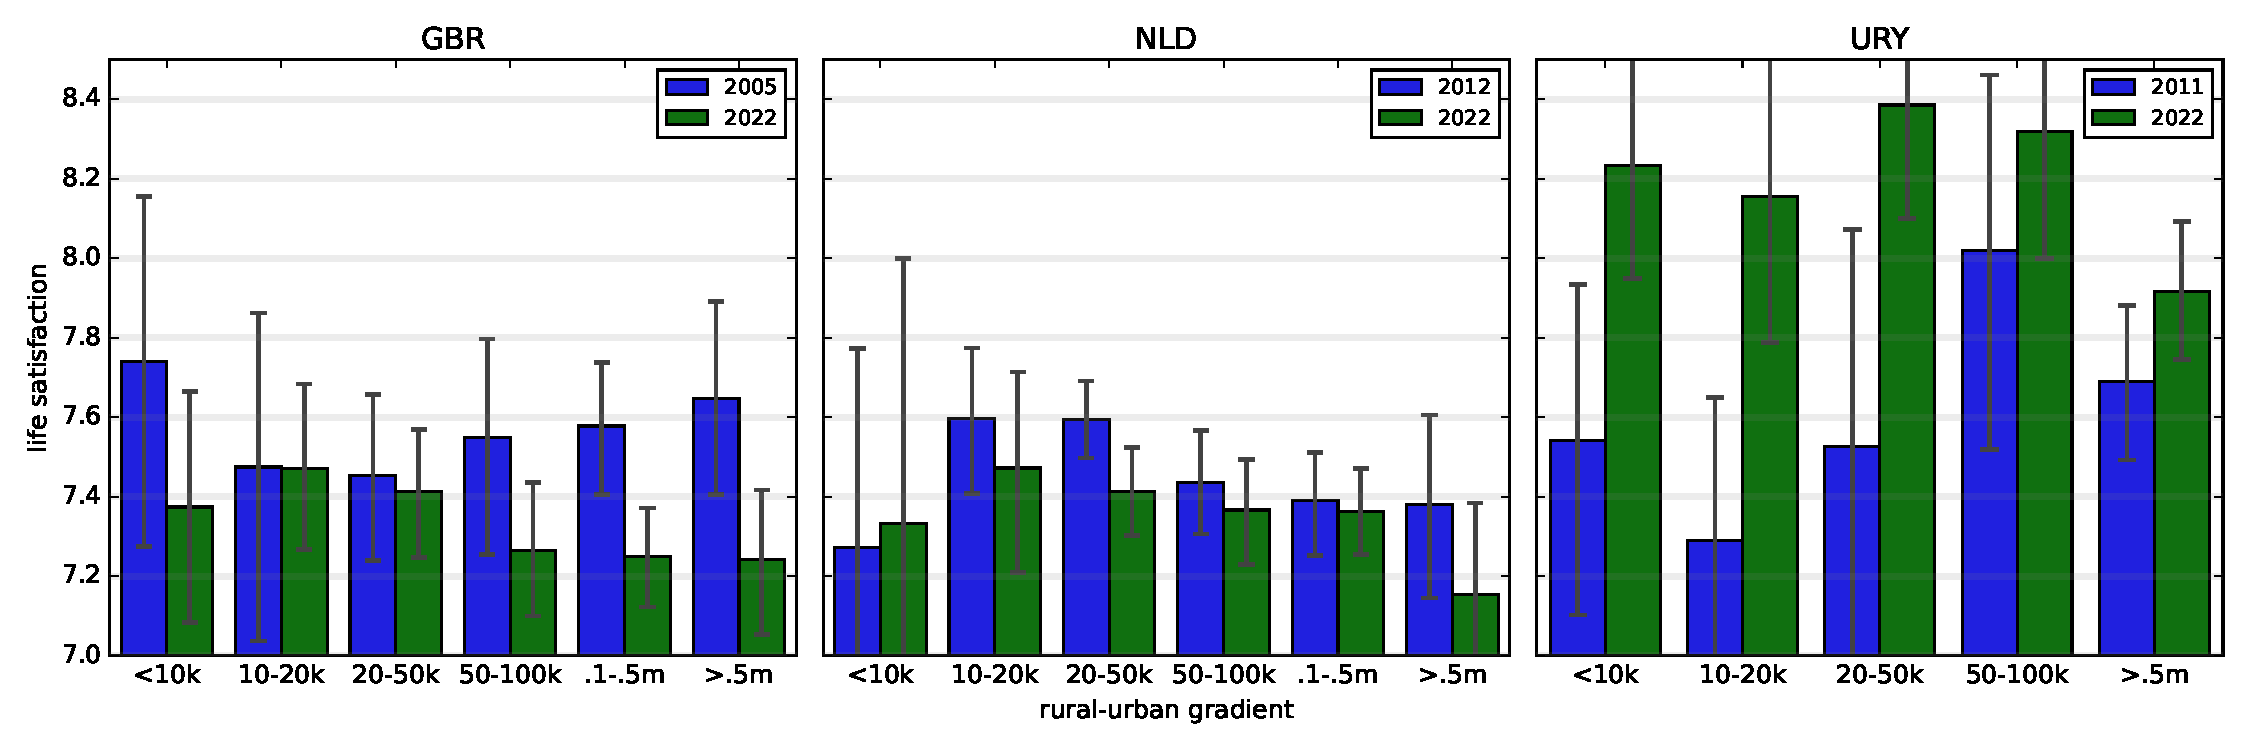
\includegraphics[width=7in]{bar.pdf}\centering
\caption{\label{bar2}Life satisfaction ($1=unhappy$ to $10=happy$) means with 95\% CI against rural urban gradient categories. $GBR=$ United Kingdom, $NLD=$ Netherlands, $URY=$ Uruguay. Note: URY is missing .1-.5m category due to small cell sizes.}
 \end{figure}

In the United Kingdom, pre-pandemic, the happiest places were the smallest
($<10k$), while during the pandemic, both the smallest and largest places were
most affected and saw significant reduction in SWB. It is unexpected to see this
reduction in the smallest places, and the result could be due to some country
specific factors (also note large confidence intervals).

In the Netherlands, there's not much change in SWB in the smaller places pre v during the pandemic, except for the largest cities where there's a larger drop in SWB as expected. There was also a smaller drop in places with 10-20k, and especially in the 20-50k categories. 

Uruguay, a developing country, shows a different story: SWB increased across urbanicity, including the largest areas ($>$.5m), but that's also where the smallest increase occurred, as expected. Many of the CI are wide, and so even large mean differences may not be
statistically significant.  
%TODO fix Figure 1, so that the CI are shown completely, it's cut off for Uruguay. meh no jaja
%RV COMMENT: LOL...i guess no reviewer complained so...you win. =)
%
%aok:yay
Next, we test the differences with OLS regression.\footnote{The usual argument in
  favor of OLS over categorical models is repeated in the online appendix. And a set
of control variables is also motivated.} First, since the focus is on cities versus smaller areas (rural and towns), for simplicity, we collapsed all categories $<$.5m into one, as rural and towns, and contrast it with cities ($>$.5m). 


There are also two technical reasons for such a binary gap approach versus using the original
gradient in the  bar charts. It is a simpler exposition to have an urban dichotomy as opposed to a gradient, given that we also have two other breakdowns: pre-during COVID, and by country. And, critically, the cell sizes run small with too many breakdowns for this relatively small dataset. When more data becomes available, future research should test the full urban-rural gradient.  

Our hypothesis is that while the pandemic decreased SWB in general, we expect to
see an even greater SWB decrease in cities. We are focused on the pre-during
pandemic differences in SWB levels in city ($>.5m$) versus smaller areas ($<.5m$). 

The bivariate regression results are in Table \ref{a}. We first separate our
analyses by country\footnote{One reason to split by country is that countries
  are diverse, and pooling them together introduces much heterogeneity, hence,
  we first proceed country-by-country, and only then introduce a pooled model.} and then within each country by rural and towns ($<.5m$) versus cities $(>.5m)$. We regress life satisfaction on a year dummy for 2022 with the base case being the latest pre-pandemic wave as shown in Figures \ref{barA} and \ref{bar2}. 
% First we could look at overall change in happiness pre-post pandemic or such % change for all areas except large cities.



\begin{spacing}{.9} \begin{table}[H]\centering   \begin{scriptsize} \begin{tabular}{p{1.8in}p{.5in}p{.5in}|p{.5in}p{.5in}|p{.5in}p{.5in}|p{.5in}p{.5in}p{.5in}p{.5
                                                                      in}p{.5in}p{.5
                                                                      in}}\hline&\multicolumn{2}{c}{GBR}&\multicolumn{2}{c}{NLD}&\multicolumn{2}{c}{URY}\\
                                                                                          &   $<.5m$   &     $>.5m$   &   $<.5m$   &     $>.5m$   &   URYrurTow   &     URYcity   \\
2022                &       -0.21** &       -0.41** &       -0.12** &       -0.23   &        0.75***&        0.23+  \\
constant            &        7.54***&        7.65***&        7.50***&        7.38***&        7.54***&        7.69***\\
N                   &        3111   &         521   &        3572   &         373   &        1154   &         836   \\

                                                                      \hline +
                                                                      0.10 *
                                                                      0.05 **
                                                                      0.01 ***
                                                                      0.001;
                                                                      robust std
                                                                      err \end{tabular}\end{scriptsize}\caption{\label{a}OLS
                                                                    regressions
                                                                    of life
                                                                    satisfaction
                                                                    on pandemic
                                                                    dummy
                                                                    (``2022'') only. WVS
                                                                   country
                                                                   samples split
                                                                 by rural and towns ($<.5m$) v cities $(>.5m).$}\end{table} \end{spacing}


The effect sizes on the year 2022 dummy are the bar length differences from Fig
\ref{barA} or \ref{bar2} for cities $(>.5m)$ and the average bar lengths for smaller
areas now collapsed as ($<.5m$). For GBR the difference pre-during pandemic is about .2 for rural areas and towns ($<.5m$), and the difference for cities $(>.5m)$ is about .4, and so
forth for the NLD and URY.
 %
 A remarkable finding in our analysis is the roughly 2 times difference for GBR (.2 v .4)
 and NLD (.1 v .2) , and 3 times difference for URY (.7 v .2)---this is a strong differential. When comparing cities $(>.5m)$ versus smaller areas ($<.5m$), cities became 2 to 3 times less happy during the pandemic compared to pre-pandemic levels.
 
Still, one of the coefficients for the NLD is not significant, and only weakly
significant for URY, and there is left out variable bias. {Differences in SWB levels should be even bigger when controlling for SWB predictors as the urban rural happiness gradient often emerges only after controlling for SWB predictors \citep{aok21}.} Hence, we elaborate our models with SWB predictors in Table \ref{b}.

\begin{spacing}{.9} \begin{table}[H]\centering   \begin{scriptsize} \begin{tabular}{p{1.8in}p{.5in}p{.5in}|p{.5in}p{.5in}|p{.5in}p{.5in}|p{.5in}p{.5in}p{.5in}p{.5
                                                                      in}p{.5in}p{.5
                                                                      in}}\hline\hline&\multicolumn{2}{c}{GBR}&\multicolumn{2}{c}{NLD}&\multicolumn{2}{c}{URY}\\
                                                                                          &   $<.5m$   &     $>.5m$   &   $<.5m$   &     $>.5m$   &   URYrurTow   &     URYcity   \\
2022                &       -0.18*  &       -0.39+  &       -0.20***&       -0.45** &        0.42***&        0.21   \\
income              &        0.09***&        0.01   &        0.06***&        0.14***&        0.07*  &        0.13***\\
age                 &       -0.03*  &       -0.08** &       -0.02+  &       -0.06+  &        0.00   &       -0.06** \\
age2                &        0.00** &        0.00** &        0.00** &        0.00*  &       -0.00   &        0.00** \\
male                &       -0.18** &       -0.13   &       -0.11*  &       -0.27+  &        0.06   &        0.19   \\
married or living together as married&        0.53***&        0.74***&        0.44***&        0.23   &        0.46** &        0.06   \\
divorced/separated/widowed&        0.07   &        0.15   &       -0.11   &       -0.14   &       -0.37+  &       -0.19   \\
autonomy            &       -0.11*  &       -0.07   &       -0.11** &       -0.01   &       -0.06   &        0.06   \\
freedom             &        0.44***&        0.42***&        0.35***&        0.43***&        0.43***&        0.36***\\
trust               &        0.12+  &        0.42** &        0.43***&        0.28+  &       -0.05   &        0.10   \\
postmaterialist     &       -0.05   &       -0.18   &       -0.11*  &        0.14   &       -0.02   &        0.15   \\
god important       &        0.01   &        0.05*  &        0.02*  &       -0.01   &        0.05** &        0.06** \\
constant            &        4.08***&        5.95***&        4.59***&        4.80***&        3.47***&        4.58***\\
N                   &        1985   &         309   &        2283   &         237   &         736   &         579   \\

                                                                      \hline +
                                                                      0.10 *
                                                                      0.05 **
                                                                      0.01 ***
                                                                      0.001;
                                                                      robust std
                                                                      err \end{tabular}\end{scriptsize}\caption{\label{b}OLS
                                                                    regressions
                                                                    of life
                                                                    satisfaction:
                                                                    added
                                                                    predictors
                                                                    of life satisfaction. WVS
                                                                   country
                                                                   samples split
                                                                 by rural and towns ($<.5m$) v cities $(>.5m)$.}\end{table} \end{spacing}

The elaborated models in Table \ref{b} mostly confirm our earlier results. We find that there's again roughly a 2 times difference for GBR and the NLD, while for URY the differential is reduced from about 3 times to roughly 2 times as well. 

As a robustness check we add ``health'' as a control variable in Table
\ref{c}. It is important to underscore that there's a confounding effect between
pre-during covid19 and health by definition. And there will also be confounding
effects between urbanicity and health since covid19 is more prevalent (at least
in initial phase) in cities as previously discussed.  Hence, these regressions are less useful in
determining pre-during difference, and the coefficients are smaller and less significant, as expected.
Remarkably though, we find that the urbanicity differentials, even though less statistically significant, are still about 2 times larger for GBR and URY and even stronger for the NLD.
%aok: this sentence doesnt make sense here lol
%rv: thats fine, lets remove, i guess we meant that on top of covid there were all of these other factors affecting SWB 
% Arguably, the high infections rate of covid19
% in cities is in addition to other urban problems such as misanthropy and
% overall malaise \citep{aok22,wilson85,rosenberg56,aok-swbGenYcity18,fischer73,fischer76}. Future research is needed.


\begin{spacing}{.9} \begin{table}[H]\centering   \begin{scriptsize} \begin{tabular}{p{1.8in}p{.5in}p{.5in}|p{.5in}p{.5in}|p{.5in}p{.5in}|p{.5in}p{.5in}p{.5in}p{.5
                                                                      in}p{.5in}p{.5
                                                                      in}}\hline\hline&\multicolumn{2}{c}{GBR}&\multicolumn{2}{c}{NLD}&\multicolumn{2}{c}{URY}\\
                                                                                          &   $<.5m$   &     $>.5m$   &   $<.5m$   &     $>.5m$   &   URYrurTow   &     URYcity   \\
2022                &       -0.12   &       -0.26   &       -0.06   &       -0.24+  &        0.44***&        0.23   \\
health              &        0.48***&        0.67***&        0.62***&        0.77***&        0.56***&        0.32** \\
income              &        0.05** &       -0.01   &        0.04***&        0.08** &        0.05   &        0.12***\\
age                 &       -0.02*  &       -0.07*  &       -0.01   &       -0.03   &        0.01   &       -0.05*  \\
age2                &        0.00** &        0.00** &        0.00** &        0.00+  &       -0.00   &        0.00*  \\
male                &       -0.16*  &       -0.15   &       -0.09+  &       -0.23+  &       -0.01   &        0.14   \\
married or living together as married&        0.49***&        0.60** &        0.38***&        0.21   &        0.41** &        0.04   \\
divorced/separated/widowed&        0.05   &        0.20   &       -0.15   &       -0.27   &       -0.36+  &       -0.16   \\
autonomy            &       -0.12** &       -0.09   &       -0.10** &        0.07   &       -0.09   &        0.04   \\
freedom             &        0.38***&        0.29***&        0.29***&        0.31***&        0.40***&        0.35***\\
trust               &        0.07   &        0.28*  &        0.34***&        0.21   &       -0.07   &        0.01   \\
postmaterialist     &       -0.05   &       -0.26+  &       -0.09*  &        0.06   &        0.01   &        0.12   \\
god important       &        0.01   &        0.02   &        0.02+  &        0.00   &        0.05** &        0.06** \\
constant            &        2.72***&        4.29***&        2.46***&        2.01*  &        1.31+  &        3.31***\\
N                   &        1985   &         309   &        2279   &         236   &         736   &         578   \\

                                                                      \hline +
                                                                      0.10 *
                                                                      0.05 **
                                                                      0.01 ***
                                                                      0.001;
                                                                      robust std
                                                                      err \end{tabular}\end{scriptsize}\caption{\label{c}OLS
                                                                    regressions
                                                                    of life
                                                                    satisfaction:
                                                                    added ``health.'' WVS
                                                                   country
                                                                   samples split
                                                                 by rural and towns ($<.5m$) v cities $(>.5m)$.}\end{table} \end{spacing}


In the online appendix we do not split by urban/rural but instead we add a urban/rural dummy
and interaction with the pandemic dummy---the interaction is statistically insignificant, i.e., the pandemic differential urban v rural effect is not statistically significant if split by country. However, if the urbanicity variable is not collapsed into the binary urban-rural, but left as several categories, the differences for the Great Britain and Uruguay are statistically significant. 
 %RV COMMENT: NICE! SO YOU FOUND THE ISSUE THEN!GOOD! 
 %
 %aok: kinda, not perfect, but something 
Finally, we pool data for the three countries together in Table
\ref{d}.
%Our final set of results shows all pooled data together. Earlier we split the sample by pre-post COVID, and large city versus town and rural areas for simplicity and ease of interpretation. However, 
 


\begin{spacing}{.9} \begin{table}[H]\centering   \begin{scriptsize} \begin{tabular}{p{1.8in}p{.5in}p{.5in}p{.5in}p{.5in}p{.5in}p{.5in}p{.5in}p{.5in}p{.5in}p{.5
                                                                      in}p{.5in}p{.5
                                                                      in}}\hline
                                                                                          &          a1   &          a2   &          a3   &          a4   &          a5   \\
post pandemic            &       -0.20** &       -0.13+  &       -0.10   &       -0.02   &       -0.18*  \\
city lg500k&        0.05   &        0.19*  &        0.20*  &        0.11   &        0.07   \\
post pandemic $\times$ city lg500k&       -0.26*  &       -0.26*  &       -0.26*  &       -0.21+  &       -0.15   \\
United Kingdom      &       -0.04   &        0.03   &        0.08   &       -0.01   &       -0.04   \\
Uruguay             &        0.82***&        0.92***&        0.95***&        0.68***&        0.43***\\
2011                &       -0.82***&       -0.72***&       -0.54***&       -0.47***&       -0.44***\\
2012                &       -0.10   &        0.15+  &        0.11   &        0.02   &        0.05   \\
income              &               &        0.14***&        0.13***&        0.08***&        0.08***\\
age                 &               &       -0.05***&       -0.04***&       -0.03***&       -0.03***\\
age2                &               &        0.00***&        0.00***&        0.00***&        0.00***\\
male                &               &       -0.16***&       -0.17***&       -0.16***&       -0.11** \\
married or living together as married&               &        0.46***&        0.46***&        0.39***&        0.44***\\
divorced/separated/widowed&               &        0.01   &        0.01   &       -0.03   &       -0.07   \\
god important       &               &               &        0.03***&        0.03***&        0.02***\\
trust               &               &               &        0.38***&        0.25***&        0.26***\\
postmaterialist     &               &               &       -0.04   &       -0.05+  &       -0.04   \\
autonomy            &               &               &       -0.10***&       -0.10***&       -0.09***\\
health              &               &               &               &        0.71***&               \\
freedom             &               &               &               &               &        0.40***\\
constant            &        7.58***&        7.42***&        7.14***&        4.40***&        4.47***\\
N                   &        9196   &        7746   &        6038   &        6032   &        5970   \\

                                                                      \hline +
                                                                      0.10 *
                                                                      0.05 **
                                                                      0.01 ***
                                                                      0.001;
                                                                      robust std
                                                                      err \end{tabular}\end{scriptsize}\caption{\label{d}OLS
                                                                    regressions
                                                                    of life
                                                                    satisfaction. Country-wave
                                                                  pooled models.}\end{table} \end{spacing}

 We start with a basic model where we regress life satisfaction on a dummy for the largest cities, and during-pandemic wave dummy where ``pandemic'' $=1$ if $year=2022$. We also include country dummies, as we now pull all the data together. We also include year dummies in addition to pandemic dummy since data were collected in different countries in different years. 

In column a1, as expected,  during the pandemic SWB went down by -.2, and
especially so for cities by an additional -.26. When adding basic controls in
model a2, ``pandemic$*$city lg 500k'' stays about the same at -.26. We include an extended
list of controls in model a3, and again the coefficient stays at -.26. It is only
after adding ``health'' in model a4 that the coefficient slightly drops to
-.21.

The addition of freedom in model a5 cuts the effect most substantially to -.15 and loses statistical significance. 
 % 
{The freedom variable comes from the following survey item: ``Some people feel they
  have completely free choice and control over their lives, while other people
  feel that what they do has no real effect on what happens to them. Please use
  this scale where 1 means 'none at all' and 10 means 'a great deal' to indicate
  how much freedom of choice and control you feel you have over the way your
  life turns out.'' A rationale to look at freedom is that it confounds with
  city; i.e., cities have more freedom than rural areas at least in some senses. The idea
  goes back at least to Ferdinand Toennies' ``Gemeinschaft und Gesellschaft'' \citep{tonnies57}--city air is free--e.g., nonstandard/nonconformist people, such as LGBTQ, are more free in an urban area.}

The WVS freedom variable also measures control over one's life. Clearly, during
  the covid19 pandemic, city residents, all things equal, would have felt a greater loss of
  control over their lives since they were more exposed to being infected. This
  may explain why  `freedom' removes the effect of the interaction variable ``pandemic
  x city lg500k.''\footnote{We thank an anonymous reviewer for providing this
    explanation. Likewise, the anonymous reviewer also points to institutional trust (the more you trust the institution the more you are confident that the COVID-19 situation is handled well by the authorities). Maybe rural residents have higher institutional trust and if
    so, maybe this could explain their lower loss of happiness. For discussion
    see \citet{sorensen2022role}. Future research could further explore freedom,
    control, and institutional trust.} 

\section{Conclusion and Discussion}

%Rural at least in the US---millennial's paper that city swb was doing better v rural arguably
%because rural has been left behind. 
The present study argues that the covid19 pandemic has lowered SWB in
large cities. % In the US, before the pandemic, city happiness was
% on the rise relative to rural areas \citep{millennials}. As rural areas have
% been left behind \citep{hansonCityJournalautumn15}, the rural happiness
% advantage has decreased. A rural Californian explains \citep[][p. 2]{fullerNYT17monD}:
%
% \begin{quote}``In the rural parts of the state we drive more miles, we drive
%   older cars, our economy is an agriculture- and resource-based economy that
%   relies on tractors. You can't move an 80,000-pound load in an electric
%   truck. They've devastated ag [agricultural] jobs, timber jobs, mining jobs with their
%   environmental regulations, so, yes, we have a harder time sustaining the
%   economy, and therefore there's more people that are in a poorer situation.''
% \end{quote}
%
% The situation may be similar in many other countries---urbanization had been
% favored over rurality in world development in general \citep{lipton77}.
%
%
% Ironically, 
The covid19 pandemic made the economic advantage and prosperity of
cities quickly wither away. The pandemic created significant economic turmoil
particularly in large urban centers: as businesses and industries shut down,
millions lost their jobs, and thousands fled to the suburbs or smaller places,
hoping to avoid human interaction and protect themselves against the
virus. Places like New York City, that were vibrant and full of life, became
dull and empty. Still, as of 2023, much of the commercial real estate in urban cores
is empty.

Urban and rural areas experienced and coped with the pandemic very
differently. Urban areas became the center of coronavirus outbreaks around the
world, and many cities saw their healthcare systems become quickly overwhelmed
given the magnitude of the virus---makeshift hospitals and makeshift morgues were
set up in urban places like New York City.

There's always a strong correlation between subjective well being and
health. Health is the key predictor of happiness---almost no one considers health
unimportant \citep[e.g.,][]{campbell76etal}. The virus not only made people
severely ill, but it prevented people who had any other health emergencies or
issues from being properly taken care of (e.g., cancer, heart disease,
diabetes). Thus, the number of people who's health was directly or indirectly affected by covid19 is significantly larger then the reported statistics of covid19 infection. This was
particularly an issue in large metropolitan areas. Covid19' impact on wellbeing is arguably larger than simply measuring it by incidence,
hospitalization, and death counts--e.g., social distancing in itself (regardless of infection) increases psychological distress \citep{khan2021quality}.
%RV COMMENT: Do you negative effect as in negative correlation? for some reason when i read it, it reads awkwardly and seems like we are saying there's a negative correlation between social distancing and psychological distress, which is wrong
%
%aok: i rephrazed
Thus, it is no surprise that our findings show such a significant and relatively
large drop in happiness levels in cities as compared to smaller places.

We interpret the impact of Covid-19 broadly, not narrowly  focused on disease
and mortality only. There is the scare inflicted by such happenings to people in the
vicinity. And there are socio-economic consequences of
  restrictions, such as unemployment. One of the standard arguments for urban
  advantage is the availability amenities such as commodities, services, and
  work/career opportunities. The opportunity to take advantage of such amenities
  is  reduced by the restrictions.  Such a
  "bundle view/domain satisfaction view" of life satisfaction is arguably
  applicable here.\footnote{We thank an anonymous reviewer for this point.}


Understanding the urban-rural discrepancies is important because policymakers can implement
policies targeted to create a more healthy and livable environment for urban and
rural residents based on the different challenges they experience to foster
happiness. The spread of infectious disease in cities is unavoidable and will
likely happen again in the near future. Learning from the challenges brought by
covid19 might result in lifesaving, health and happiness promoting measures.


It is important to highlight that only the initial phase of an infection per capita
is greater in cities, then urban versus rural rates converge, and in the last stage,
infections are higher in rural areas as cities get hit first and recover first
\citep{cuadros2021dynamics}---at least in the US---and we assume that elsewhere
the mechanism will be similar. 

But there is arguably a strong psychological effect, urban scare, that will also last well beyond the pandemic in the foreseeable future---future research can test it. Likewise, urban quality of life versus rural quality of life even given
similar\footnote{Assuming similar per capita rates is not illogical: cities experience increased infection rate only initially, but then infection
  rates in smaller areas rise as cities recover and disease
  spreads to smaller areas.} per capita infection is very different---one can easily go about daily life and even enjoy most rural activities in rural areas, while the opposite is true in cities---the urban way of life is unbearable during a pandemic.


The massive difference in population density of urban versus rural needs to be
underscored. The disproportionate population density signifies that even if the infection rate were similar across urban-rural areas, the difference in infection rate per sq km would be
massive. And this is one key factor behind the urban scare from covid19---the sheer number of
infections in one's proximity was astronomical.

The pandemic has brought attention to the many problems of the cities. 
In many ways, cities cannot be fixed---there is an inherent conflict, dysfunction
and even misanthropy in metropolis \citep{wirth38,fischer72,aok22,thrift05,amin06,aokCityBook15,peck16}. 
 %
Others would argue that a city can be fixed and made happier \citep[for a review
see][]{ballas13}. An useful discussion of directions for change is \citet{olasov22}---for
instance, to re-imagine cities as places that offer convivial and sensual shared space for shared pleasure, ``a mesh of small, safe, intimate places, rather than a series of grand urban projects.''


\section{Limitations and Future Research}

These are the first  analyses examining the urban-rural SWB differential during the covid19 pandemic. As such, there are limitations that need to be considered. First, even though population size and density correlate, they are not the same---future research
could use density to explore whether these findings are robust. Unfortunately, the WVS only measures urbanicity by population size, and we know that the spread of infectious diseases like covid19 and the subjective ``urban scare'' are not only due to population size, but also density. 

In addition, there may be time effects---covid19 developed differently in different places over
time---see covid19 trajectories in the online appendix. We only used 2 periods for each
country---before and during the pandemic. Another dataset that has more time points would be
useful to test the robustness of these findings.

{One potential threat to identification is that slower diffusion of infectious disease to rural areas compared to urban areas
may have affected the results. Another threat is omitted
variables, although we have strived to mitigate it with multiple
specifications including before-after (pre and during pandemic)
 2 group (urban v rural) specification, so called difference-in-difference (DID). Also note that study of urbanization is inherntly observational,
not experimental (or even quasi-experimental).}

As more data becomes available, it will be instructive to closely examine
countries that were most affected by covid19. The results from Great
 Britain, the Netherlands, and Uruguay studied here may not generalize to other
 countries, especially ones with much different covid19 rates, policy responses
 and urbanization patters. Italy and the U.S., for example,
will probably show much greater negative effects on SWB than what we found in
the UK (GBR), the Netherlands (NLD) and Urguguay (URY). Although covid19
infection rates are significantly lower now (in 2023),
and another massive pandemic could be decades ahead, we'll likely experience
covid19 lingering effects for many years to come. This could arguably include
urban scare, prevalence of misanthropolis (a metropolis full of distrust and
dislike of humankind) \citep{aok22}, and possibly an urban crisis. It would be
useful to study the long term effect on urban-rural happiness gradient/gap and whether covid19
has widened more permanently the urban-rural happiness gap that had been closing prior to the pandemic
\citep{aok-swbGenYcity18}.

This is only the first study on the topic and more research is needed to examine
the impact of covid19 on the urban-rural gradient/gap. We are interested in the
general and overall patterns we observed here and believe it provides a good
starting point for a much needed debate on this topic. Future research can focus
on a more direct link between infections, hospitalizations, and deaths and SWB
by linking public health data with SWB data for specific locations. Likewise
there is a huge difference in infection rates across countries (e.g., Italy, the
US, China), and across places within countries. Such differences could be
perhaps explored in a natural experiment framework where massively infected area
can be matched with a similar area but with low infection rate.


% \section*{\Huge ONLINE APPENDIX}
% \textbf{[note: this section will NOT be a part of the final version of
%   the manuscript, but will be available online instead]} %hence everything below
%                                 %is organized byu section, not subsection
% !!!
% have most of the stuff outputted to online appendix:)--start with that and then
% select stuff to paper--have brief narrative describng patterns in online app too
% !!!

% \section*{Variables' definitions, coding, and distributions}
% \label{app_var_des}


% %\input{/tmp/a.tex} %aok_var_des

% % \begin{spacing}{.9}
% %   \begin{table}[H]\centering \caption{Summary statistics.} \label{sumSta} \begin{scriptsize} \begin{tabular}{p{1.8in}p{.5in}p{.5in}p{.5in}p{.5in}p{.5in}p{.5in}p{.5in}p{.5in}p{.5in}p{.5
% %             in}p{.5in}p{.5 in}}\hline
% %         \input{/tmp/aha2.tex}
% %          \end{tabular}\end{scriptsize}\end{table}
% % \end{spacing}

% % \begin{spacing}{.9}
% %   \begin{table}[H]\centering \caption{Correlation matrix.} \label{sumSta} \begin{scriptsize} \begin{tabular}{@{}
% %           p{1.2in} rrrrrrrrrrrrr @{}}\hline
% %         \input{/tmp/ahb2.tex}\hline
% %          \end{tabular}\end{scriptsize}\end{table}
% % \end{spacing}



% Table XXX shows variable distributions. If a variable has more than
% 10 categories it is classified into bins...

% %\input .... %TODO !!!! have input here histograms

% \section*{Additional Descriptive Statistics}
% \label{app_des_sta}

% %make sure i have [H] or h! ???
% % \begin{table}[H]
% % \caption{}
% % \centering
% % \label{}
% % \begin{scriptsize}
% % \input{../out/reg_c.tex}
% % \end{scriptsize}
% % \end{table}

%\newpage
%\theendnotes
\bibliography{/home/aok/papers/root/tex/ebib.bib,covidCity.bib}

\section{Online Appendix}

\textbf{[note: this section is appended in the manuscript for ease of peer
  review; it will NOT be a part of the body of the final version of  the
  manuscript, but will be linked from it and  available online instead]} %hence everything below


\subsection{Variable Definitions and Distributions}

\input{varDes.tex}

\input{hist.tex}

Finally, below detailed distributions aka crosstabs by country and then by
urbanicity and wave. 

\begin{scriptsize}
\begin{spacing}{.85}
\begin{verbatim}
. ta X049 yr if cc=="GBR"
ta X049 yr if cc=="GBR"

                   |      Year survey
   Settlement size |      2005       2022 |     Total
-------------------+----------------------+----------
        under 2000 |         6         18 |        24 
            2-5000 |        18         96 |       114 
           5-10000 |        34         92 |       126 
          10-20000 |        80        289 |       369 
          20-50000 |       264        494 |       758 
         50-100000 |       133        419 |       552 
        100-500000 |       378        800 |     1,178 
   500000 and more |       128        397 |       525 
-------------------+----------------------+----------
             Total |     1,041      2,605 |     3,646 

. ta X049 yr if cc=="NLD"
ta X049 yr if cc=="NLD"

                   |      Year survey
   Settlement size |      2012       2022 |     Total
-------------------+----------------------+----------
            2-5000 |         2          2 |         4 
           5-10000 |        20         10 |        30 
          10-20000 |       187         92 |       279 
          20-50000 |       691        647 |     1,338 
         50-100000 |       414        465 |       879 
        100-500000 |       419        598 |     1,017 
   500000 and more |       169        217 |       386 
-------------------+----------------------+----------
             Total |     1,902      2,031 |     3,933 

. ta X049 yr if cc=="URY"
ta X049 yr if cc=="URY"

                   |      Year survey
   Settlement size |      2011       2022 |     Total
-------------------+----------------------+----------
        under 2000 |        11         60 |        71 
            2-5000 |        39         40 |        79 
           5-10000 |        57         80 |       137 
          10-20000 |       118         90 |       208 
          20-50000 |        55        140 |       195 
         50-100000 |        54        120 |       174 
        100-500000 |         1         30 |        31 
   500000 and more |       398        440 |       838 
-------------------+----------------------+----------
             Total |       733      1,000 |     1,733 
\end{verbatim}
\end{spacing}
\end{scriptsize}

  
\subsection{Model and Controls}

We use a standard OLS regression with robust standard errors.  We treat the 10-step
happiness variable as continuous. Ordinal happiness can be treated as a
continuous variable \citep{carbonell04}.
%
OLS has become the default method in happiness research
\citep{blanchflower11}. Theoretically, while there is still debate about the
cardinality of SWB, there are strong arguments to treat it as a cardinal
variable \citep{ng96,ng97}. 


In the choice of controls, we generally follow \citet{aok21}. There are specific
controls worth discussing.  One great advantage of city living that is often forgotten is freedom,  ``City air makes men free (Stadt Luft macht frei)'' \citet[p. 12]{park84}\footnote{It
   originated in the Middle Ages, and it meant freedom from feudalism,
   non-feudal islands in a sea of feudalism \citep{harvey12}.}, hence we control
 for freedom. Health is a key predictor of SWB, and also note that the subjective health measure used here is a reasonable measure of actual health \citep{subramanian09b}.

More discussion regarding the control choice of freedom is in the paper at the end of the results section. 

\subsection{Covid Trends in GBR, NLD, URY}

Ideally, we would like to see trends by settlement size, but these are best and most
cross-country consistent data we have found---data from \url{https://coronavirus.jhu.edu/region}.

 \begin{figure}[H]
  \includegraphics[height=3in]{jhuGbr.pdf}\centering\label{jhuGbr}
 \caption{GBR}
 \end{figure}

  \begin{figure}[H]
  \includegraphics[height=3in]{jhuNld.pdf}\centering\label{jhuNld}
 \caption{NLD}
 \end{figure}

  \begin{figure}[H]
  \includegraphics[height=3in]{jhuUry.pdf}\centering\label{jhuUry}
 \caption{URY}
 \end{figure}

\subsection{Policy Responses in GBR, NLD, URY}

The key policy is vaccination. 
The three countries were relatively highly vaccinated at 75\% or more (the
timeline is missing in the datasource). \% of Population receiving at least 1 dose from \url{https://coronavirus.jhu.edu/region/}:\\
GBR 79\\
URY 87\\
NLD 75\\

Next, social distancing and closure measures. There are substantial measures in
place for all three countries ranging from partial or receommended restrictions
to full or/and necessary restrictions.\\

Social Distancing and Closure Measures from \url{https://www.kff.org/report-section/global-covid-19-tracker-policy-actions/}\\

\begin{table}[H]
  \centering
  \begin{tabular}{p{2cm}p{2cm}p{2cm}p{2cm}p{2cm}p{2cm}p{2cm}p{2cm}}
    Country&Cancel public events&Stay at home&Workplace closing&School closing&Restrictions on gatherings&Restrictions on internal movement&Intl travel controls\\
    United Kingdom&Require cancelling&No restriction&Partial closing&Partial closing&Full restriction&Internal movement restrictions in place&Partial restriction\\
    Uruguay&Recommend cancelling&Recommend not leaving house&Partial closing&Partial closing&Partial restriction&Recommend not to travel between regions/cities&Full restriction\\
Netherlands&Require cancelling&Recommend not leaving house&Partial closing&Partial closing&Full restriction&Recommend not to travel between regions/cities&Partial restriction\\
  \end{tabular}
  \caption{Social Distancing and Closure Measures.}
\end{table}

Furthermore, from the same datasource, the United Kindgdom citizens have received broad support in terms
of both income support and debt contract relief. The Netherlands citizens have received broad support in terms
of income support, but narrow support in terms of debt contract relief. The
least amount of support took place in Uruguay: some support in terms
of income support, narrow support in terms of debt contract relief.

In terms of  Health Systems Measures, still from the same datasource, both
United Kingdom and Netherlands in terms of Vaccination Eligibility and 	Facial
Coverings score respectively: Partial availability and Recommended/Partial requirement.
 The difference for Uruguay is in terms of Vaccination Eligibility: ``Universal
 availability,'' thus potentially explaining the highest vaccination rate in
 Uruguay, about 10\% higher than in the other two countries. 	

The most elaborate information\footnote{Still, we could not find urban-rural
  details, a pertinent informatoion for the present study, and limitation.} on policy responses come from\\
\url{https://www.imf.org/en/Topics/imf-and-covid19/Policy-Responses-to-COVID-19},
which is cited below. The big advantage is information on the timeline of
responses. It is not straightforward to compare this mostly qualitative
information. While all three countries produced significant policy responses,
the United Kingdom and the Netherlands are much richer countries per capita than Uruguay
and hence even similar resources in terms of percent of GDP are higher.\\


United Kingdom
\begin{scriptsize}
\begin{spacing}{.85}
\begin{verbatim}

Background. The first confirmed case was reported on January 31, 2020. Cases
initially peaked in April/May, and after weeks of decline, a second and third
waves took hold with the number of cases significantly above those seen during
the initial peak. In response to the initial outbreak, on March 23 the
government implemented a range of measures including travel restrictions, social
distancing measures, closures of entertainment, hospitality, non-essential shops
and indoor premises, and increased testing. The largest economic hit was in
2020Q2 when GDP fell by 19.5 percent q-o-q, reflecting a sharp contraction in
April. Overall, the UK's economy contracted by 9.8 percent in 2020. Frictions in
implementing the post-Brexit trade regime will also weigh on activity in the
short run. Even after social distancing winds down, a period of corporate
balance sheet repair is expected to weigh on investment while labor reallocation
takes place gradually. The pre-crisis level of output would be recovered in
early-2022 but output would remain about 3 percent below the pre-2020 trend in
2025.


Reopening of the economy. On May 10, 2020, the government set out a roadmap to
ease the lockdown in England (Scotland, Wales, and Northern Ireland have
separate rules).Reopening took place in three steps starting on May 13 and
continuing through July, with educational facilities reopening in September.The
relapse of infections led initially to localized restrictions based on a 3-tier
system of intensity, but eventually a second country-wide lockdown was put in
place on November 5 (similar restrictions were established in Scotland, Wales,
and Northern Ireland). Educational facilities, construction, and manufacturing
remained open.


New restrictions. On January 4, 2021, amidst rising contagions and the rapid
spread of a new string of the virus, PM Boris Johnson imposed a third
coronavirus lockdown across England, moving it up to tier 4, shutting schools,
restaurants, bars, and non-essential shops and ordering the public to stay at
home. Northern Ireland, Scotland, and Wales also went into lockdown. The full
emergency lockdown is being lifted in phases, starting with the reopening of
schools and recreation in outdoor public spaces on March 8. Non-essential
retail, shops, hairdressers, gyms, and outdoor hospitality reopened on April 12
in England. On May 17, outdoors most social contact rules were lifted and indoor
hospitality and hotels reopened. The final phase--full reopening--was postponed
from June 21 to July 19 on account of a new Covid wave triggered by the Delta
variant.



Key Policy Responses as of June 3, 2021

FISCAL
Tax and spending measures to support households and families during the health
emergency include: (i) additional funding for the NHS, public services, and
charities (GBP48.5billion); (ii) measures to support businesses (GBP29billion),
including property tax holidays, direct grants for small firms and firms in the
most-affected sectors, and compensation for sick pay leave; and (iii)
strengthening the social safety net to support vulnerable people (GBP8 billion)
by increasing payments under the Universal Credit scheme as well as expanding
other benefits. The government launched three separate loans schemes to
facilitate business' access to credit. Through the British Business Bank, the
Coronavirus Business Interruption Loan Scheme supports SMEs and the Coronavirus
Large Business Interruption Loans Scheme supports bigger firms, which carry an
80 percent guarantee for loans up to GBP5 million for the former and up to
GBP300 million for the latter. In addition, the government put in place the
Bounce Bank loan scheme for SMEs with 100 percent guarantee for loan amounts up
to GBP50,000. It also deferred VAT payments for the second quarter of 2020 until
the end of the financial year and income tax payments of the self-employed by
six months. The government paid 80 percent of the earnings of self-employed
workers (Self Employment Income Support Scheme, SEISS) and furloughed
(Coronavirus Job Retention Scheme, CJRS) employees (to a maximum of GBP2,500 per
employee per month) initially for the period March-May. For furloughed
employees, the scheme was extended until end-October. From July employers were
allowed to furlough employees for part of the daily working hours. Government
coverage fell to 70 percent of wages in September (up to GBP2,187) and 60
percent in October (up to GBP1,875) with employers required to contribute the
difference to 80 percent of wages (up to GBP2,500). The scheme for the
self-employed was extended for three more months but at a reduced level of 70
percent of earnings. Trade credit insurance for business-to-business
transactions received up to GBP10 billion of government guarantees through the
Trade Credit Reinsurance scheme, with the scheme available for nine months. The
government put in place a GBP1bn package to support firms driving innovation and
development through grants and loans. To support the international response, the
government made available GBP150 million to the IMF's Catastrophe Containment
and Relief Trust and provided a new GBP2.2 billion loan to the IMF Poverty
Reduction and Growth Trust (PRGT) to help low income countries respond to
COVID-19. See also:
\url{https://www.gov.uk/government/publications/guidance-to-employers-and-businesses-about-covid-19/covid-19-support-for-businesses}.


In July 2020, the government adopted a package of measures to protect and create
jobs and support the economic recovery. These include: providing firms GBP1,000
per furloughed employee retained until end-January; paying the minimum wage for
25 hours per week for six months for young workers at risk of long-term
unemployment; increased resources to enhance skills and facilitate reinsertion
in the job market; temporary reductions of the VAT rate for hospitality,
accommodation and attractions and the real estate transactions tax; increased
public spending on infrastructure (including on green projects such as
retrofitting houses to improve energy efficiency); and a program to subsidize
dining out during the month of August. Low-income people who need to
self-isolate and are unable to work, as well as members of their household, will
receive GBP130 and GBP182, respectively. Businesses required to shut down due to
localized lockdowns will receive up to GBP1,500 every three weeks.


A package of measures announced on September 24 entailed the following: (i)a
6-month Job Support Scheme (JSS) whereby employers will pay the wages of staff
for the hours they work while for the hours not worked the government and the
employer will each pay one third of their equivalent salary, up to GBP697.92 per
month each. Employees must be working at least 33 percent of their usual hours;
(ii) Extending the Self Employment Income Support Scheme for those continuing to
actively trade but face reduced demand due to coronavirus, with the initial lump
sum covering20 percent of three months' worth of profits for the period from
November to the end of January next year up to a total of GBP1,875 (an
additional second grant, will be available for the period from February 2021 to
the end of April); (iii) extending the temporary 15 percentage point VAT cut
(from 20 to 5 percent) for the tourism and hospitality sectors to the end of
March next year; (iv) allowing to pay VAT payments deferred until end-March to
be paid in 11 installments and self-assessed income tax due in July 2020 and
January 2021 to be paid in 12 installments, (v) extending the maturity of loans
under the CBILS and BBLs to up to 10 years; and (vi) extending the application
period for loans under the CBILS, CLBILS, and BBLS until end-November. In
addition, the government launched a new program, Job Entry: Targeted Support
(JETS), to help the job search of people receiving unemployment benefits for at
least 13 weeks.


Some of the measures announced in the September package were subsequently
modified to be consistent with the tighter containment measures.For businesses
that stay open, the JSS was modified, with minimum worked hours reduced to 20
percent, the government paying 62 percent for non-worked hours and employers
paying 5 percent of non-worked hours. For businesses required to close due to
the restrictions, the government will pay two thirds of the employees' salaries
(or 67 percent) up to a maximum of GBP2,100 a month, and the employers will
cover social contributions. The scheme ran for 6 months from November 1.The
value of the grant for self-employed was increased from 20 to 40 percent of
profits, up to GBP3,750. The grant for businesses required to close was
increased to up to GBP3,000 per month for businesses in England, while
additional funds were allocated to the devolved administrations. Businesses in
the hospitality, accommodation and leisure sectors in high alert areas will
receive grants of up to GBP2,100.


In view of the second lockdown, the government launched a new package of
measures in November, including the following: postponing the JSS, canceling the
Job Retention Bonus, extending the CJRS until end-March 2021 with the
replacement ratio back at 80 percent, increasing the grant of the SEISS also to
80 percent of earnings, and prolonging the deadline to apply for government
guaranteed loans until end-January 2021. On December 17, the government
announced that it would extend the furlough scheme and the business support
program one more month, until April 2021.


On November 25, the government published the 2020 Spending Review setting
expenditure limits for FY2021-22, while the OBR presented its revised fiscal
outlook. For FY2020-21, Covid-19 support measures were estimated at GBP280
billion. For FY2021-22, the government allocated GBP55 billion for this
purpose. Among other uses, these funds will be allocated to Covid testing, PPE
and vaccines, as well as the new 3-year Restart scheme to help the long term
unemployed find work.


On January 5, 2021,a day after the government imposed its toughest Covid-19
restrictions since last spring (expected now to last until at least March 8),
Chancellor Sunak announced a GBP4.6bn fresh financial support package for
struggling UK companies. This would be divided in two parts: GBP4bn of one-off
"top-up grants" for an estimated 600,000 retail, hospitality, and leisure
companies, which can each claim up to GBP9,000; and a new GBP594m discretionary
fund made available for councils to support other businesses that were not
eligible for those grants but were affected by the restrictions.


On March 3, Chancellor Sunak announced an additional fiscal stimulus of GBP59bn
(nearly 2.6 percent of GDP). This is split in virus-related support measures
worth an extra GBP43bn for this year, complimented by additional GBP15.7bn of
measures to boost the recovery. Support for households included a six-month
extension to the furlough scheme (although this will be tapered from July) worth
around GBP20bn (the self-employment part of this was more generous than expected
at GBP13bn alone). Other measures included a six-month extension to the uplift
to universal credit benefit payments (GBP2.2bn), an extension of the full cut in
VAT for the hospitality sector (GBP5bn) to the end of September (as well as a
phased return back to normal by April next year), a three-month extension of the
current stamp duty cut to the end of June (as well as a phased return to normal
by the end of September), and a freeze in alcohol and fuel duty
(GBP1.1bn). Additional funding in the form of business grants was offered
(GBP5bn), discounted business rates were extended to the end of this year
(GBP6bn), and this was accompanied by a generous tax break for businesses that
aims to encourage future investment to be brought forward to this year and next
(which the OBR estimates will cost GBP12bn). Future tax increases centered
mostly on a 6-percentage point rise in corporation tax (from 19 to 25 percent)
in 2023, and a freeze in income tax thresholds.


MONETARY AND MACRO-FINANCIAL
Key measures include: (i) reducing Bank Rate by 65 basis points to 0.1 percent;
(ii) expanding the central bank's holding of UK government bonds and
non-financial corporate bonds by GBP450 billion (in three tranches announced in
March, June, and November); (iii) introducing a new Term Funding Scheme to
reinforce the transmission of the rate cut, with additional incentives for
lending to the real economy, and especially SMEs; (iv) HM Treasury and the BoE
have agreed to extend temporarily the use of the government's overdraft account
at the BoE to provide a short-term source of additional liquidity to the
government if needed; (v) launching the joint HM Treasury-Bank of England Covid
Corporate Financing Facility and three government loan guarantee schemes-- the
Coronavirus Business Interruption Scheme, the Coronavirus Large Business
Interruption Scheme, and the Bounce Back Loan Scheme--replaced by the Recovery
Loan Scheme from April 6, 2021, providing a total of GBP352bn of liquidity and
loan guarantees available to businesses (19.5 percent of GDP); (vi) activating a
Contingent Term Repo Facility to complement the Bank's existing sterling
liquidity facilities; (vii) together with central banks from Canada, Japan, Euro
Area, U.S., and Switzerland, further enhancing the provision of liquidity via
the standing US dollar liquidity swap line arrangements; (viii) maintaining
banks' Systemic Risk Buffer (SRB) rates at the rate set in December 2019, until
at least December 2022, with any decision on the rates taken in December 2022
taking effect from January 2024; and (ix) reducing the UK countercyclical
capital buffer (CCyB) rate to 0 percent from a pre-existing path toward 2
percent by December 2020, with guidance that it will remain at 0 for at least 12
months. In December 2020, the Financial Policy Committee (FPC) updated its
guidance on the path for the CCyB rate, expecting this rate to remain at 0
percent until at least 2021 Q4. Due to the usual 12-month implementation lag,
any subsequent increase of the rate is not expected to take effect until 2022 Q4
at the earliest. See also: \url{https://www.bankofengland.co.uk/coronavirus}. On
February 3, 2021, the Bank of England finalized a technical review of the
potential impact of a negative policy rate, concluding that this could be of use
with further preparations. On March 3, 2021, the government announced the
introduction of a new mortgage guarantee scheme from April 2021 for borrowers
with a deposit of just 5 percent on homes with a value of up to GBP600,000,
together with the extension of the stamp duty land tax (SDLT) exemption until
June 2021. On April 23, 2021, the central banks have decided to discontinue
offering dollar liquidity at the 84-day maturity, given improvements in
U.S. dollar funding conditions (operational change effective as of July 1,
2021). They will however continue to hold weekly operations with a 7-day
maturity.


The Prudential Regulatory Authority (PRA) set out supervisory expectation in
March 2020 that large banks should suspend dividends and buybacks until
end-2020, cancel outstanding 2019 dividends and pay no cash bonuses to senior
staff. In December 2020, the PRA however announced its intention to return
toward the standard framework for bank distributions, reflecting some reduction
in the uncertainty related to Covid at this time, and the ability of banks to
withstand significant losses, according to results of the two stress tests
carried by the Prudential Regulation Committee (PRC) and the FPC. The PRA
indicated all Pillar 2A requirements will be set as a nominal amount, instead of
a percentage of total Risk Weighted Assets (RWAs) and to mitigate the
possibility of procyclical market risk capital requirements, the PRA will
temporarily allow firms to offset the increase in risk-weighted assets due to
the automatic application of a higher VaR multiplier through a commensurate
reduction in risks-not-in-VAR (RNIV) capital requirements (see
\url{https://www.bankofengland.co.uk/coronavirus/information-for-firms}). The
Financial Conduct Authority (FCA) introduced a package of targeted temporary
measures to support customers affected by coronavirus, including by setting the
expectation for firms to offer a payment freeze on loans and credit cards for up
to three months. In November, the mortgage moratorium was extended until
end-April and the FCA also extended for 6 months the period to request a payment
deferral for consumer credit.


On February 2021, the BoE reminded to the eight major UK banks of the importance
of the first RAF submissions (Resolvability Assessment Framework). Note in this
respect that the dates of these submissions, initially announced in May 2020 by
the BoE and the PRA had been extended by a year (from the first Friday in
October 2020, to the first Friday in October 2021), to alleviate operational
burdens on banks during the COVID-19 crisis.


EXCHANGE RATE AND BALANCE OF PAYMENTS
No measures.
\end{verbatim}
\end{spacing}
\end{scriptsize}


The Netherlands
\begin{scriptsize}
\begin{spacing}{.85}
\begin{verbatim}

Background. In response to a first wave of COVID-19 infections in late February
2020, the authorities adopted a series of sanitary measures, including a partial
lockdown to limit the spread of the virus. Following a progressive easing of
these measures from May 11, and the resurgence in the number of infections,
several containment measures with gradual restrictions were announced
successively on August 6, August 18, September 25, October 2, October 14, and
November 4.


After a second and more severe wave of infections started late in the summer
2020, the number of infections surged again toward the end of the year,
prompting the authorities to impose the strictest lockdown since the beginning
of the pandemic. All non-essential businesses, schools (with few exceptions),
daycares, and many public spaces such as parks and zoos were ordered to
close. It was required to work from home unless not possible, avoid public
transportations, limit gatherings to one guest from a different household (three
during Christmas celebrations), maintain social distancing, and strongly advised
not to travel abroad. These restrictions initially in place from December 15 to
February 9, were subsequently extended through April 27. A curfew from 9 pm to
4:30 am was also introduced (from January 23 to April 27). In addition, a
negative PCR test was required for travelers to the Netherlands from high-risk
countries.


On March 3, a few restrictions were lifted to allow partial reopening of primary
and secondary schools. This was followed by a progressive reopening strategy, as
infections and hospital admissions declined steadily and vaccines became widely
available (as of June 30, 2021, about 15.5 million doses of vaccines have been
administered), Under the first phase starting on April 28, the curfew was
lifted, restaurants and cafés were allowed to operate outdoor, and shops to
reopen at limited capacity, among other measures. Additional restrictions were
lifted in a second phase from May 19, including the use of public
transportations, travel to certain destinations, and hours of operations for
some businesses. Under the third phase starting on June 05, restaurants and
cafes can operate indoor, cinemas and other larger cultural institutions can
reopen, all under strict conditions (including for example maintaining 1.5
meters social distancing). From June 26, the fourth phase allows all businesses
to operate at their regular hours, with a requirement to maintain a 1.5 meters
distance or to wear a face mask, except if vaccinated. The advice to work from
home and restrictions to group gathering are lifted. Several travel restrictions
are also lifted.



Key Policy Responses as of July 1, 2021

FISCAL
A series of fiscal measures have been introduced since the start of the pandemic
to contain the economic impact of the outbreak. The two first support packages
(announced in March and May, respectively) include spending measures estimated
at about 35.3 billion euros (4.4 percent of GDP) in 2020, and covering (i)
compensation of up to 90 percent of labor costs for companies expecting a
reduction in revenues of 20 percent or more; (ii) compensation for affected
sectors (hospitality, travel, agriculture, culture, and others); (iii) support
for entrepreneurs and the self-employed, start-ups and small innovation
companies; (iv) scaling up of the short-time working scheme (unemployment
benefit compensation available to companies needing to reduce their staff by at
least 20 percent), (v) allowances for SMEs to help them finance their fixed
costs. In addition, companies can defer tax payments without penalties, and
calculate provisional taxes on the basis of expected reduced activity levels. In
2020, revenue shortfalls from deferral of tax payments and other forgone revenue
measures are estimated at 17.2 billion euros (or 2.2 percent of GDP). Also,
public guarantee schemes (with a ceiling increased by 65 billion euros, or 8.1
percent of GDP), especially for SME loans but also covering large firms, are
expanded to help the most vulnerable companies to manage their liquidity
problems. A guarantee scheme for supplier credit has also been established. On
August 28, the government announced the third support package which primarily
aims at expanding and adjusting measures already in place on the expenditure
side through June 2021. The authorities also aim at supporting labor mobility
toward expanding sectors. Platforms to facilitate job transition are being
developed, and public financing is being allocated for training, re-skilling and
career counseling. Tax incentives are also introduced to support private
investment. In 2020, expenditure support amounted to 27.8 billion (or 3.4
percent of GDP), and the government has budgeted a 40.9 billion (or 4.7 percent
of GDP) support package in 2021.


MONETARY AND MACRO-FINANCIAL
The ECB decided to provide monetary policy support through (i) additional asset
purchases of EUR120 billion until end-2020 under the existing program (APP), and
(ii) providing temporarily additional auctions of the full-allotment, fixed rate
temporary liquidity facility at the deposit facility rate and more favorable
terms on existing targeted longer-term refinancing operations (TLTRO-III)
starting between June 2020 and June 2021. Further measures included an
additional EUR750 billion asset purchase program of private and public sector
securities (Pandemic Emergency Purchase Program, PEPP) until end-2020, an
expanded range of eligible assets under the corporate sector purchase program
(CSPP), and relaxation of collateral standards for Eurosystem refinancing
operations (MROs, LTROs, TLTROs).


The ECB Banking Supervision allowed significant institutions to operate
temporarily below the Pillar 2 Guidance, the capital conservation buffer, and
the liquidity coverage ratio (LCR). In addition, new rules on the composition of
capital to meet Pillar 2 Requirement (P2R) were front-loaded to release
additional capital. The ECB considers that the appropriate release of the
countercyclical buffer by the national macroprudential authorities will enhance
its capital relief measures. The ECB Banking Supervision further decided to
exercise -- on a temporary basis -- flexibility in the classification requirements
and expectations on loss provisioning for non-performing loans (NPLs) that are
covered by public guarantees and COVID-19 related public moratoria; it also
recommended that banks avoid pro-cyclical assumptions for the determination of
loss provisions and opt for the IFRS9 transitional rules. More recently, ECB
Banking Supervision asked banks to not pay dividends for the financial years
2019 and 2020 or buy back shares during COVID-19 pandemic, from which the
conserved capital should be used to support households, small businesses and
corporate borrowers and/or to absorb losses on existing exposures to such
borrowers.


In addition, the Dutch central bank has reduced systemic buffer requirements for
the three largest banks to support bank lending. The central bank is also taking
measures to provide temporary regulatory relief to less significant banking
institutions.Banks under direct supervision of DNB are also allowed to exclude
specific central bank exposures when calculating their leverage
ratios. Furthermore, the planned introduction of a floor for mortgage loan risk
weighting was initially postponed; however, the May 2021 Financial Stability
Report announced that this floor would be introduced on January 1, 2022. The
largest Dutch banks grant SMEs a six-month postponement of their loan
repayments. To protect homeowners, the government and relevant stakeholders
agreed that there will be no mortgage foreclosures until July 1 2020. From July
1st, homeowners facing financial difficulties are encouraged to contact their
lender to renegotiate more flexible terms for the period covering the ongoing
economic crisis. On October 6, 2020, the authorities adopted a law to facilitate
debt restructuring for companies facing financial difficulties. The law is
intended to prevent bankruptcies.


EXCHANGE RATE AND BALANCE OF PAYMENTS
No measures.
\end{verbatim}
\end{spacing}
\end{scriptsize}


Uruguay
\begin{scriptsize}
\begin{spacing}{.85}
\begin{verbatim}

Background. The first cases of COVID-19 were reported on March 13, 2020. The
government introduced a series of public health measures, such as school
closures, cancellation of public events, and active discouragement of large
gatherings. Starting April 22, customers must wear face masks while shopping in
supermarkets; this rule is currently being expanded to other
establishments. International travel has been severely restricted. After months
of relative stability, the number of new infections has increased sharply in
November.Daily new cases have increased exponentially since Q4 2020, surpassing
450 per million as of end-March (higher than in neighboring Brazil), although
the death count remains relatively low. The recent surge likely reflects limited
movement restrictions in late 2020 and the emergence of the highly contagious
P.1 variant in Brazil, as the two countries share a porous border.


Reopening of the economy. Construction activity was allowed to restart in
mid-April of 2020, government offices re-opened in early May, and shopping
centers reopened on June 9, all with appropriate sanitary precautions. Bars and
restaurants are reopening, and the soccer matches began in August, without the
spectators. As of June 29, almost all schools (including in the capital
Montevideo) have been re-opened. Starting August 3, school hours were extended
to be closer to normal hours. Borders, however, will remain largely closed for
the foreseeable future. However, amid the recent steep rise in COVID-19 cases,
there is growing public pressure to impose stricter lockdown measures. Borders
have been closed since December 2020, in-person schooling is suspended,
government offices closed, and the population encouraged to stay home.


Vaccination. Vaccination started on March 1, 2021 and is one of the fastest
rollouts in the region, next to Chile, reflecting the efficient registration
setup via web and mobile apps. The government has secured around 5.5 vaccine
doses and about 18 percent of the population has received at least one dose of
vaccine as of end-March. The government plans to get the entire population
vaccinated in the 1 half of 2021 on a voluntary basis.



Key Policy Responses as of June 3, 2021

FISCAL
Additional resources to address the public health emergency have been mobilized,
including by resorting to contingent credit lines from other international
financial institutions. In 2020, the overall above-the-budget-line fiscal cost
has been estimated at $800 million (1.6 percent of GDP). The measures include
(i) relaxation of rules for claiming the unemployment insurance (0.8 percent of
GDP); (ii) expanded assistance to the most vulnerable groups (cash and direct
provision of food, 0.2 percent of GDP); (iii) expanded sick leave benefits,
including for older workers, so they do not have to leave home (0.1 percent of
GDP). Furthermore, some tax and pension obligations are being postponed or
reduced and utility payments are being cancelled or reduced for some
companies. Starting in June, the government subsidized employment by paying
companies 5,000 pesos per month (about 1/3 of the current minimum wage) for
three months for each new hire. As a solidarity measure, the salaries of
better-paid public officials are being reduced by up to 20 percent, with the
savings directed to the newly-established Coronavirus Fund. Other sources for
the Coronavirus Fund include the additional Social Security Assistance Tax, the
2019 profits of Banco República and the National Development Corporation, and
donations. Currently, this fund finances the cash subsidies and food assistance
for the most vulnerable, together with the cash subsidies for the employees in
the construction industry affected by the pandemic-related work stoppages. In
March 2021, the government announced an extension of some of the measures,
including extension of credit guarantees and unemployment insurance, tax relief
for small businesses; increase in assistance to the most vulnerable; and
extension of investment incentives.In April 2021, the government announced that
it plans to spend $900 million (1.6 percent of GDP) in Covid-related measures
during 2021. It also complemented existing measures with a 6-month suspension of
social security contributions for SMEs in sectors most affected by the pandemic
(e.g.; tourism, hotels, restaurants etc).


MONETARY AND MACRO-FINANCIAL
The central bank has been focused on maintaining the appropriate level of
liquidity in the system. It has temporarily reduced the reserve requirements
that apply to the nominal peso and the inflation-adjusted peso deposits in the
commercial banks. This measure has injected about USD 150 million of additional
liquidity into the financial system.


The central bank has temporarily relaxed the regulations in the securities and payments markets and extended the deadlines for data submission.

Loan payments for households and businesses that occur between March 1 and August 31, 2020 are to be deferred for up to 180 days.

The fund that guarantees loans for SMEs has been expanded from USD 50 million to
USD 500 million (utilizing financing from international organizations). That is
expected to allow to guarantee the SME loans up to USD 2.5 billion. In addition,
the rate of commission charged by the fund will be reduced
substantially. Moreover, two more guarantee lines are being established, one for
larger enterprises and another for enterprises in the sectors (such as tourism)
that are directly affected by border closures.


BROU (the country's largest commercial bank, which is government-owned) will
extend soft loans to enterprises. The financing available currently is USD 50
million, which may be augmented--also with financing from international
organizations--to USD 120 million. In addition, direct credit program for micro
and small enterprises will extend working capital loans of up to 18 months to
the affected businesses at subsidized rates. Loan repayments for these
enterprises are being suspended for at least 30 days. 


EXCHANGE RATE AND BALANCE OF PAYMENTS
The exchange rate has been allowed to adjust, with the central bank intervening to limit undue volatility in the market.
\end{verbatim}
\end{spacing}
\end{scriptsize}

 

\subsection{Interaction or Pandemic Dummy with Urban/Rural Dummy Separately for
  Each Country}
 
In Table \ref{a}, we repeat the previous 3 sets of models, but instead of splitting
by urban/rural, we add an interaction to test if the pandemic urban rural difference
is statistically significant, and it is not. The sign and effect sizes are as expected. 


\begin{spacing}{.9} \begin{table}[H]\centering   \begin{scriptsize} \begin{tabular}{p{1.8in}p{.5in}p{.5in}p{.5in}|p{.5in}p{.5in}p{.5in}|p{.5in}p{.5in}p{.5in}p{.5 in}p{.5in}p{.5 in}}\\ \input{/tmp/regABC.tex} \hline + 0.10 * 0.05 ** 0.01 *** 0.001; robust std err \end{tabular}\end{scriptsize}\caption{\label{abc}OLS regressions of life satisfaction.}\end{table} \end{spacing}

However, having more gradation in urbanicity, produces more statistical 
significance in table \ref{regX}. The rationale is to use more/fuller information on
urbanicity. And with regressions, the rationale is also to have a large stable base case, here
$<50k$, and compare it against the 3 larger places $50-100$, $100-500$, $gt500$ 

\begin{scriptsize}
\begin{spacing}{.85}
\begin{verbatim}
                   |                    town3
   Settlement size |         1          2          3          4 |     Total
-------------------+--------------------------------------------+----------
        under 2000 |        95          0          0          0 |        95 
            2-5000 |       197          0          0          0 |       197 
           5-10000 |       293          0          0          0 |       293 
          10-20000 |       856          0          0          0 |       856 
          20-50000 |     2,291          0          0          0 |     2,291 
         50-100000 |         0      1,605          0          0 |     1,605 
        100-500000 |         0          0      2,195          0 |     2,195 
   500000 and more |         0          0          0      1,749 |     1,749 
-------------------+--------------------------------------------+----------
             Total |     3,732      1,605      2,195      1,749 |     9,281 
\end{verbatim}
\end{spacing}
\end{scriptsize}


\begin{spacing}{.9} \begin{table}[H]\centering   \begin{scriptsize} \begin{tabular}{p{1.6in}p{.45in}p{.45in}p{.45in}|p{.45in}p{.45in}p{.45in}|p{.45in}p{.45in}p{.45in}p{.5 in}p{.45in}p{.5 in}}\\ \input{/tmp/regX.tex} \hline + 0.10 * 0.05 ** 0.01 *** 0.001; robust std err \end{tabular}\end{scriptsize}\caption{\label{regX}OLS regressions of life satisfaction.}\end{table} \end{spacing}

%RV COMMENT: I would remove the next section, reviewer didn't like it, and not sure it really proves anything....some people get sick, some don't...more likely to get sick, but maybe we should just comment it out ?
%
%aok: ok
%\subsection{Anecdotal Evidence: An Author Got Covid}

% Many people think that covid19 is largely gone and cities are safe to return
% to. One of the authors of this study was reckless enough to go to a large city,
% New York City, and surely enough just got infected with covid19 this summer
% (2023) when we were revising this paper. We advise the readers to keep away from
% large cities--you will be safer from infectious disease and happier.

% But then again, this is anecdotal. An anonymous reviewer also got covid19, but
% outside of a large city. 

 \subsection{Morocco (MAR) and  Venezuela (VEN)}


Morocco (MAR), like Uruguay (URY) in the body of the paper, increased SWB everywhere, but
least in the largest cities ($>$500k), and also in 100-500k category. The 20-50k
category should not be interpreted as there are only 22 observations in 2001, (and 0 obs
in the 50--10k category).

In the case of Venezuela (VEN), most places had a drop in SWB, and while larger places had a little more drop than smaller ones, there are no clear patterns unlike in other
countries. And this is not surprising. Venezuela, like Morocco, only had a little proportion of
its population affected by covid, about 2-3 percent. But unlike Morocco, it is a
non-free autocracy with an unstable/turbulent economy---we did not expect to see
much of an effect of covid in Venezuela.  

 \begin{figure}[H]
  \includegraphics[height=3in]{marVen.pdf}\centering\label{marVen}
 \caption{Urban-rural happiness gradeint in Morocco and Venezuela pre and during
 the pandemic.}
 \end{figure}


\section{Urbanism and infectious disease spread}

 \begin{figure}[H]
  \includegraphics[height=3in]{bettencourt.pdf}\centering\label{marVen}
 \caption{\citet{bettencourt21}}
 \end{figure}



\end{spacing}
\end{document}
